\documentclass[11pt,a4paper]{article}
\usepackage[T1]{fontenc}
\usepackage[utf8]{inputenc}
\usepackage{lmodern}
\usepackage{amsmath}
\usepackage[margin=2.3cm]{geometry}
\usepackage{booktabs}
\usepackage{tabularx}
\usepackage{longtable}
\usepackage{array}
\usepackage[table,dvipsnames]{xcolor}
\usepackage{graphicx}
\usepackage{float}
\usepackage{enumitem}
\usepackage{titlesec}
\usepackage{parskip}
\usepackage{setspace}
\usepackage{needspace}
\usepackage{caption}
\usepackage[hidelinks]{hyperref}

\setstretch{1.15}
\setlength{\parskip}{0.6em}
\setlist{itemsep=0.25em, topsep=0.3em}
\renewcommand{\arraystretch}{1.3}
\captionsetup{font=small, labelfont=bf}
\definecolor{accent}{RGB}{31,78,95}
\definecolor{ok}{RGB}{21,128,61}
\definecolor{part}{RGB}{180,83,9}
\definecolor{no}{RGB}{185,28,28}
\titleformat{\section}{\Large\bfseries\color{accent}}{\thesection}{0.8em}{}
\titleformat{\subsection}{\large\bfseries}{\thesubsection}{0.8em}{}
\titlespacing*{\section}{0pt}{1.4em}{0.6em}
\titlespacing*{\subsection}{0pt}{1.0em}{0.35em}
\newcolumntype{L}{>{\raggedright\arraybackslash}X}
\newcolumntype{P}[1]{>{\raggedright\arraybackslash}p{#1}}
\newcommand{\file}[1]{\texttt{\small #1}}
\newcommand{\MET}{\textcolor{ok}{\textbf{Met}}}
\newcommand{\PART}{\textcolor{part}{\textbf{Partly}}}
\newcommand{\NOT}{\textcolor{no}{\textbf{Not yet}}}
\newcommand{\dep}{\rowcolor{gray!18}}
\newcommand{\answer}[1]{\par\noindent\colorbox{accent!8}{\parbox{\dimexpr\linewidth-2\fboxsep}{\vspace{0.4em}\textbf{Answer.} #1\vspace{0.4em}}}\par}

\begin{document}

% =====================================================================================================
\begin{titlepage}
\centering
\vspace*{2.2cm}
{\large Indian Institute of Information Technology, Allahabad\par}
{\large Department of Information Technology\par}
\vspace{2.2cm}
{\Huge\bfseries\color{accent} TinyIDS\par}
\vspace{0.8em}
{\LARGE Lightweight, Explainable Intrusion Detection\\[0.2em] for IoT Gateways\par}
\vspace{1.2em}
{\large Internet of Things: Term Project Report\par}
\vspace{2.2cm}
{\large\bfseries Group 10\par}
\vspace{0.6em}
\begin{tabular}{ll}
\toprule
Name & Enrolment No. \\
\midrule
Ayush Gupta & MWC2025013 \\
Sanket Maroti Bodhe & MWC2025005 \\
Meharvan Verma & MWC2025012 \\
Akshit Rawat & MWC2025011 \\
Alekhya China & MCL2025011 \\
Pritam Chaudhary & IIT2023102 \\
Yash Kamthan & IIT2023149 \\
\bottomrule
\end{tabular}
\vfill
{\large November 2026\par}
\vspace{1cm}
\end{titlepage}

% =====================================================================================================
\section*{Abstract}

IoT gateways are the natural place to stop attacks on cheap, poorly secured devices, but they lack the compute for
heavy intrusion detection, and most published IoT IDS results stop at workstation accuracy. TinyIDS is a
lightweight, explainable intrusion detection and prevention system that runs in real time on a Raspberry Pi~4
gateway. A single LightGBM model classifies every window of 10 packets per sender as Benign, Flood or Recon from
14 header features that the gateway computes exactly as in the CICIoT2023 dataset; simple rules add DoS-vs-DDoS
counting, port-scan, MQTT brute-force and spoofing detection; every alert is explained by its top-3 TreeSHAP
features; attackers are blocked automatically through the Linux firewall. On the full CICIoT2023 test split the
model reaches a binary F1 of 0.997 with 0.97\% false alarms; on the Pi it uses 974~KB, 0.7--1.4~ms per decision,
5--14~ms per SHAP explanation and 77--78~MB of RAM, meeting every efficiency target of the proposal. In a live
MQTT testbed with three NodeMCU sensors, every attack (six flood types, a three-node botnet DDoS, scans and
brute force) was detected and blocked with zero false alarms on the sensors.

\tableofcontents
\vspace{0.6em}
\noindent\colorbox{gray!18}{\strut\ Grey rows\ } in all tables = the model deployed on the Raspberry Pi
(LightGBM, 3 classes, 14 features, 974 KB).

\newpage
% =====================================================================================================
\section{Introduction}

\subsection{Motivation}

Cameras, smart plugs and sensors ship with weak security and are routinely recruited into botnets (Mirai-style
DDoS, brute force, reconnaissance). They all communicate through a gateway, which is therefore the natural place to
detect and stop attacks. Gateways, however, are small devices, and few published IoT IDS measure whether a model
fits a real gateway's latency and memory budget, or explain why an alert fired.

\subsection{Problem statement and research questions}

Design an intrusion detector that runs in real time on a Raspberry Pi~4 gateway, uses a small set of traffic
features, and gives a human-readable reason for every alert.

\begin{itemize}
  \item \textbf{RQ1:} How few flow features (out of 46 in CICIoT2023) keep macro-F1 within 2\% of the full model?
  \item \textbf{RQ2:} Which compressed model (tree ensemble, pruned MLP, small 1D-CNN) gives the best accuracy per
        millisecond and per megabyte?
  \item \textbf{RQ3:} Can SHAP explanations be produced on the gateway fast enough to accompany live alerts?
\end{itemize}

\subsection{Contributions}

\begin{enumerate}
  \item A deployed IDS + IPS on a Raspberry Pi~4: one 974~KB LightGBM model, rule-based detectors and automatic
        firewall mitigation, with every alert explained by TreeSHAP.
  \item A feature set chosen for \emph{validity}: only the 14 features our gateway computes identically to the
        dataset, verified by recording our own attacks.
  \item A benchmark of four classifiers (RF, LightGBM, MLP, 1D-CNN) on binary, 8- and 34-class tasks, a feature-count
        study (RQ1) and a compression study (RQ2).
  \item A live MQTT testbed (Pi, 3 NodeMCUs, attacker laptop, botnet) and a reproducible Docker copy of it.
\end{enumerate}

% =====================================================================================================
\section{System design}

\subsection{High-level design}

The testbed is five devices on one Wi-Fi network (Figure~\ref{fig:hld}). Three NodeMCU (ESP8266) sensors publish
readings over MQTT to a Mosquitto broker on the Raspberry Pi. The same Pi runs the TinyIDS detector, which captures
every packet sent to it, and the Linux firewall that enforces its decisions. The laptop runs the operator dashboard
and the bot master (Windows) and the attack tools (WSL).

\begin{figure}[H]
\centering
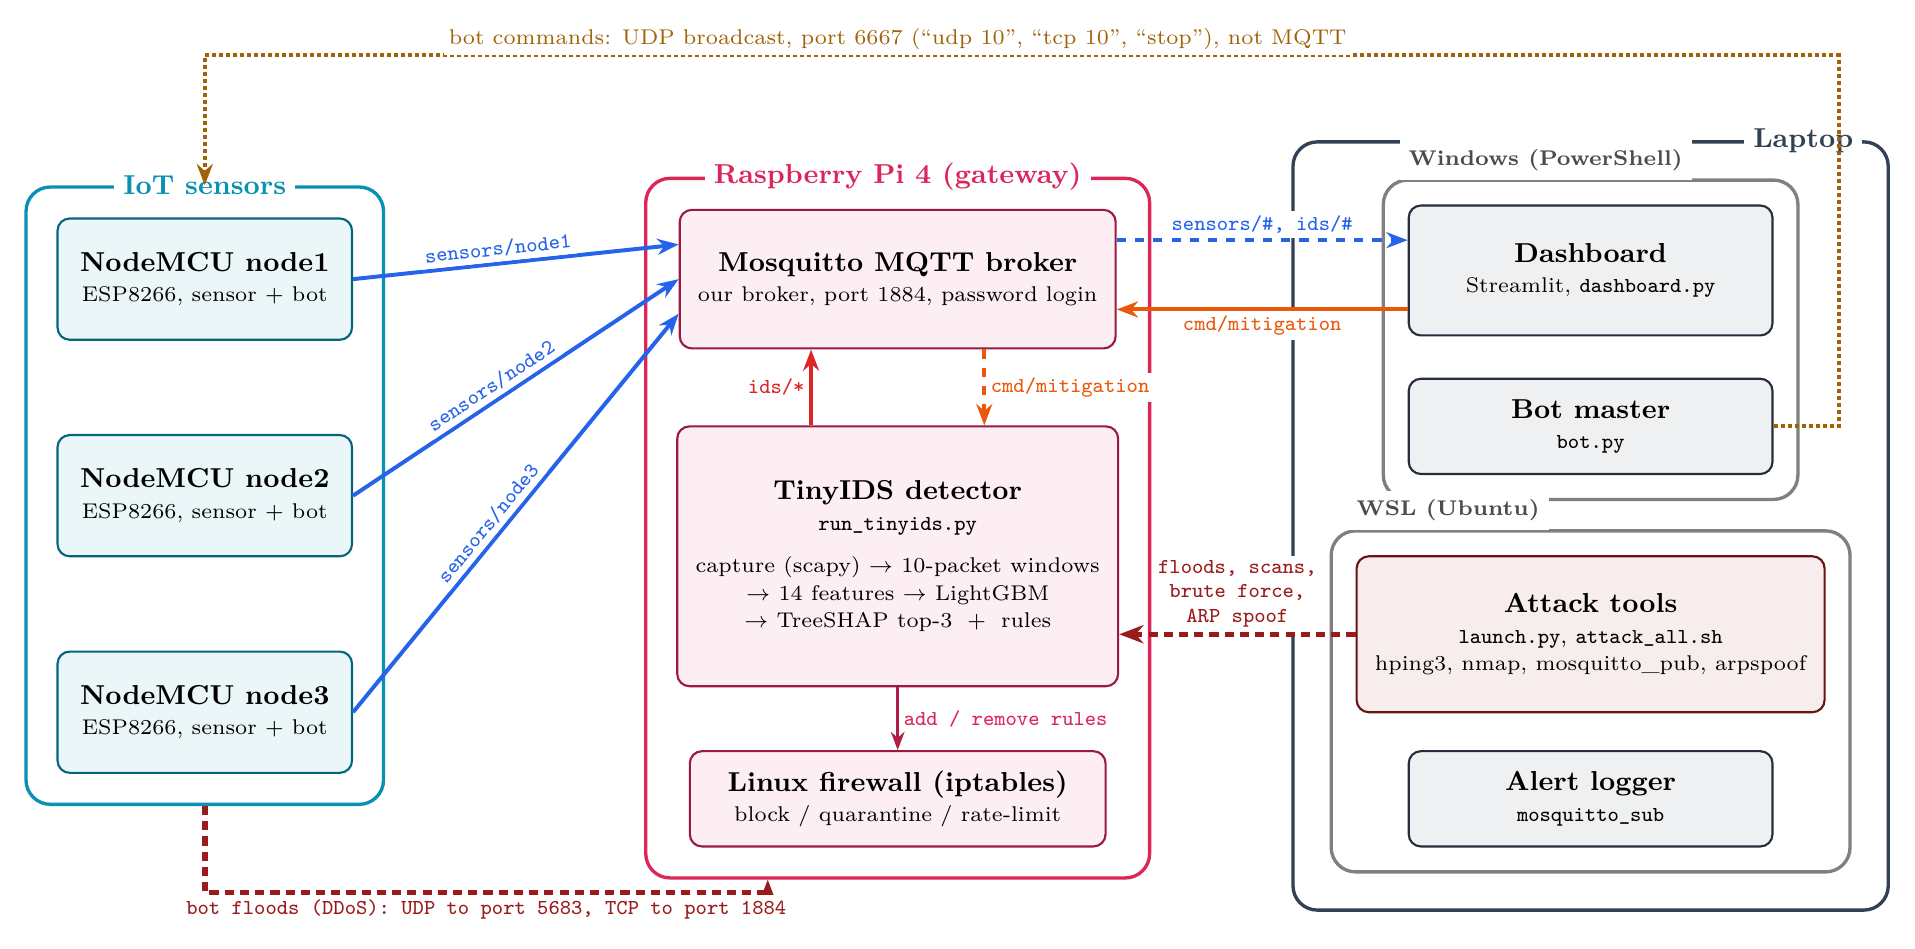
\includegraphics[width=\linewidth]{../ppts/assets/hld.png}
\caption{High-level design. Solid arrows: MQTT messages published to the broker; dashed: delivered to a
subscriber; red: attack traffic; brown: bot commands.}
\label{fig:hld}
\end{figure}

\subsection{Communication: MQTT topics}

\begin{center}
\small
\begin{tabularx}{\linewidth}{P{3.6cm}P{2.4cm}P{2.6cm}L}
\toprule
Topic & Publisher & Subscriber & Content \\
\midrule
\file{sensors/<node>} & each NodeMCU & dashboard & temperature, humidity, every 2 s \\
\file{ids/alerts} & detector & dashboard, logger & attack, confidence, top-3 SHAP reasons, timings \\
\file{ids/stats} & detector & dashboard & packets/s, windows, model and SHAP time, every second \\
\file{ids/mitigation/status} & detector & dashboard & blocked / quarantined / rate-limited IPs (retained) \\
\file{ids/status} & detector & dashboard & model, features, start time (retained) \\
\file{cmd/mitigation} & dashboard & detector & IPS on/off, release all blocks \\
\bottomrule
\end{tabularx}
\end{center}

The broker listens on TCP port 1884 and requires a login. Bot commands are not MQTT: a UDP message to port 6667.

\subsection{The detector}

\begin{figure}[H]
\centering
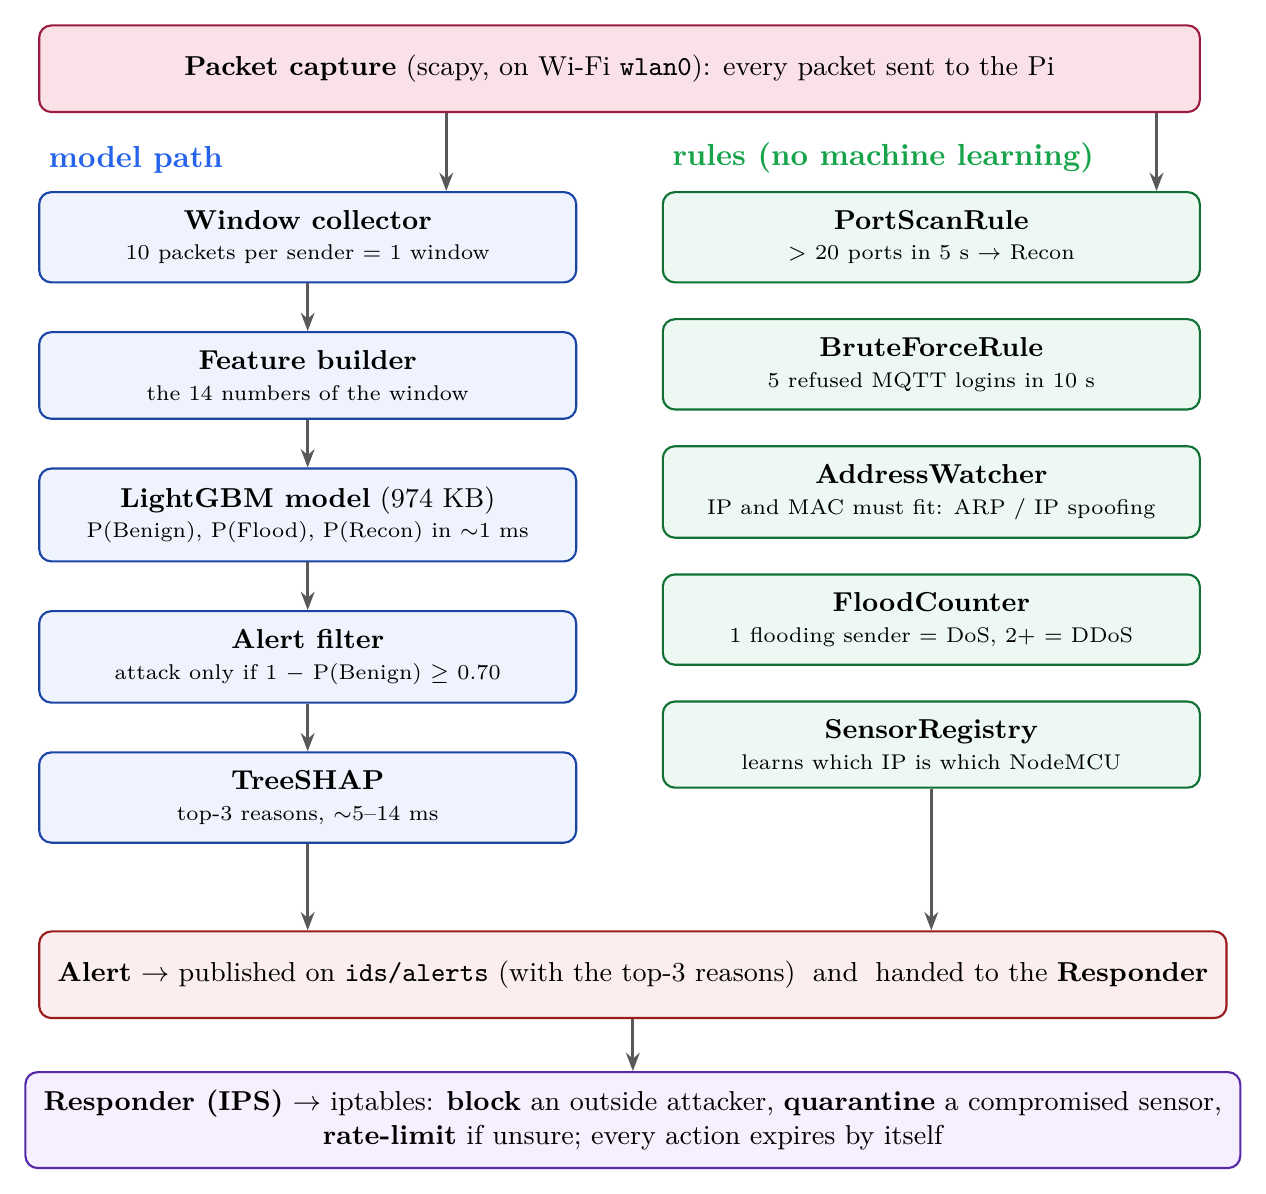
\includegraphics[width=0.82\linewidth]{../ppts/assets/detector.png}
\caption{Detector pipeline on the Pi: the model path and the rules run on every packet in parallel.}
\end{figure}

\textbf{Mitigation.} Detection happens in user space; enforcement in the kernel through \texttt{iptables}:

\begin{center}
\small
\begin{tabularx}{\linewidth}{P{2.4cm}P{5.6cm}L}
\toprule
Action & When & Effect \\
\midrule
Block & confidence $\geq$ 0.90 or a rule, outside machine & drop all packets of the source IP for 30 s \\
Quarantine & sure attack from one of our sensors & drop for 120 s, then 30 s grace for its reconnect \\
Rate-limit & 0.70--0.90, two windows in a row & drop only packets above 20/s for 30 s \\
MAC block & spoofing (the IP is fake) & drop the network card, fix the ARP entry \\
\bottomrule
\end{tabularx}
\end{center}

All actions expire by themselves; the operator laptop's SSH and dashboard connection are never blocked; SYN cookies
are enabled at start.

\subsection{Security scope by layer}

\begin{center}
\small
\begin{tabularx}{\linewidth}{P{2.6cm}P{5.4cm}L}
\toprule
OSI layer & Attacks covered & Defence \\
\midrule
2 Data link & ARP spoofing & AddressWatcher rule, MAC block \\
3 Network & ICMP flood, spoofed-source floods, DDoS & model + FloodCounter + AddressWatcher \\
4 Transport & SYN, ACK, PSH-ACK, RST-FIN, UDP floods; port scans & model + PortScanRule + SYN cookies \\
7 Application & MQTT brute force & BruteForceRule \\
\bottomrule
\end{tabularx}
\end{center}

% =====================================================================================================
\section{Data and methodology}

\subsection{Dataset}

CICIoT2023: 7.85 million rows (70/15/15 train/validation/test, as published), 46 features, 34 labels; only 2.36\%
benign. We keep \textbf{13 labels} in \textbf{3 classes}: Benign; Flood (DoS and DDoS SYN, UDP, ICMP, TCP, PSH-ACK,
RST-FIN); Recon (port, OS and vulnerability scans). The 21 others are left out: web attacks and HTTP floods need a
web server the gateway does not run; Mirai needs real malware; spoofing and brute force are handled by rules;
ping sweeps never fill a 10-packet window; fragmentation and SynonymousIP floods were not testable on our testbed.
DoS and DDoS are merged because a single row cannot show the number of senders; a rule counts them instead.

\subsection{Features}

Only the \textbf{14 features} our gateway computes exactly as the dataset does were used (verified by recording our
own floods and comparing value ranges): \file{Protocol Type}, \file{TCP}, \file{UDP}, \file{ICMP}, the shares of
the SYN, ACK, PSH, RST and FIN flags, and the packet sizes \file{Min}, \file{Max}, \file{AVG}, \file{Std},
\file{Tot size}. The other 32 are computed differently live (e.g.\ \file{Rate}, \file{Header\_Length}), are
shortcuts (\file{IAT}, the capture time), or are constant for our attacks. This addresses the proposal's validity
note directly.

\subsection{Training}

\begin{center}
\small
\begin{tabularx}{\linewidth}{P{3.4cm}P{5.2cm}L}
\toprule
Setting & Value & Reason \\
\midrule
Training data & 20\% stratified sample (909,368 rows) + 36,255 own rows & more rows gave no gain (Section 5.6) \\
Model & LightGBM, 15 leaves, 63 bins, 189 trees & small, fast, exact TreeSHAP \\
Early stopping & 20 rounds on the validation split & avoids overfitting \\
Class weights & $\sqrt{N / (3 n_c)}$: Benign 4.68, Flood 0.83, Recon 10.86 & 96\% of rows are floods \\
Decision & attack if $1 - P(\text{Benign}) \geq 0.70$ & fewer false alarms \\
Size cap & $<$ 1 MB (974 KB reached) & proposal target \\
\bottomrule
\end{tabularx}
\end{center}

Our own rows come from 25 recordings (Docker testbed and real lab) made with the detector's own feature code.
For testing they are split by \textbf{time}: in every recording the first 70\% train, the next 15\% validate, the
last 15\% test, so test windows are not near-copies of training windows.

\subsection{Evaluation metrics}

Precision, recall (detection rate) and F1 per class; macro-F1 (unweighted mean over classes, so a weak small class
counts fully); binary metrics for attack vs benign including false-positive rate (false alarms), false-negative
rate and ROC-AUC; and on the Pi: model size, peak RAM, latency per window, SHAP latency per alert.

% =====================================================================================================
\section{Results against the proposal targets}

\begin{center}
\small
\begin{tabularx}{\linewidth}{P{3.0cm}P{3.0cm}LP{1.5cm}}
\toprule
Metric & Target & Result & Status \\
\midrule
\dep Binary F1 & $\geq$ 0.98 & \textbf{0.997} on 973,829 test rows & \MET \\
\dep False-positive rate & reported & 0.97\% (dataset); 0 false alarms live on 3 sensors & \MET \\
8-class macro-F1 & within 2\% of full & 30 of 45 features suffice (RQ1) & \MET \\
\dep Model size & $<$ 1 MB & \textbf{974 KB} & \MET \\
\dep Peak RAM (Pi) & $<$ 100 MB & \textbf{77--78 MB} under attack & \MET \\
\dep Latency (Pi) & $<$ 5 ms & \textbf{0.7--1.4 ms} per window & \MET \\
\dep Throughput & $\geq$ 500 flows/s & $\approx$700--1,400 windows/s (derived from latency) & \PART \\
Energy & mJ per inference & not measured (no USB power meter) & \NOT \\
\dep SHAP latency (Pi) & $<$ 50 ms & \textbf{5--14 ms} per alert & \MET \\
\bottomrule
\end{tabularx}
\end{center}

% =====================================================================================================
\section{Evaluation of the deployed model}

\subsection{CICIoT2023 test split (973,829 rows, never used in training)}

\begin{center}
\small
\begin{tabular}{lrrrr}
\toprule
Class & Rows & Precision & Recall & F1 \\
\midrule
\dep Benign & 27,709 & 0.827 & 0.990 & 0.901 \\
\dep Flood & 940,692 & 1.000 & 0.997 & 0.998 \\
\dep Recon & 5,428 & 0.560 & 0.287 & 0.380 \\
\midrule
\dep Accuracy / macro-F1 / weighted-F1 & & \multicolumn{3}{r}{0.993 / 0.760 / 0.992} \\
\bottomrule
\end{tabular}
\hspace{1.2em}
\begin{tabular}{lr}
\toprule
Attack vs benign & Value \\
\midrule
\dep Accuracy & 0.9938 \\
\dep Precision (attack) & 0.9997 \\
\dep Recall / detection rate & 0.9939 \\
\dep F1 (attack) & 0.9968 \\
\dep False-positive rate & 0.0097 \\
\dep False-negative rate & 0.0061 \\
\dep ROC-AUC & 0.9986 \\
\bottomrule
\end{tabular}
\end{center}

\begin{figure}[H]
\centering
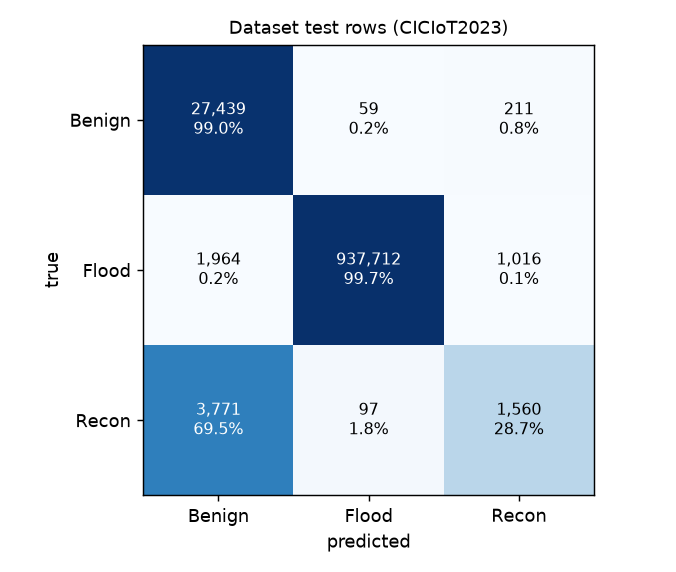
\includegraphics[width=0.46\linewidth]{images/cm_dataset_test.png}
\hfill
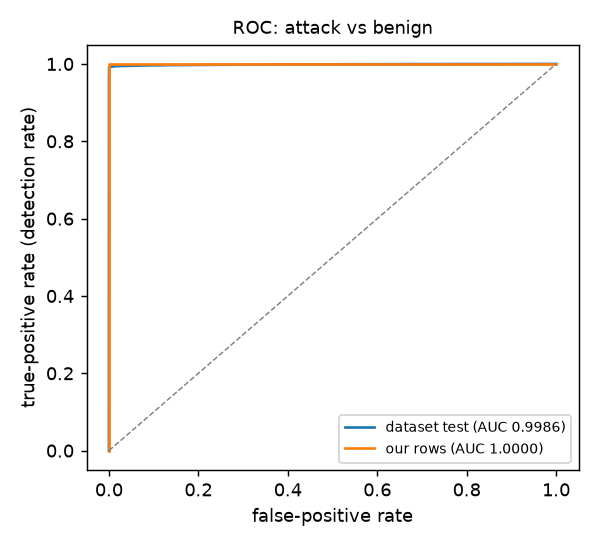
\includegraphics[width=0.46\linewidth]{images/roc_attack_vs_benign.png}
\caption{Left: confusion matrix on the dataset test split. Right: ROC curve, attack vs benign, dataset test split
and our own traffic.}
\end{figure}

Floods are detected almost perfectly. Recon is the weak class: most dataset scan rows look like benign traffic in
these 14 features (3,771 of 5,428 scan rows are called Benign).

\subsection{Every dataset attack label}

Detection rate per label on the test split, including the 21 labels the model was never trained on.

\begin{center}
\small
\begin{tabular}{lrr@{\hspace{2.2em}}lrr}
\toprule
Trained label & Rows & Detected & Not-trained label & Rows & Detected \\
\midrule
DDoS-ICMP\_Flood & 180,447 & 99.9\% & DDoS-SynonymousIP\_Flood & 90,480 & 99.9\% \\
DDoS-UDP\_Flood & 136,717 & 99.8\% & Mirai-greeth\_flood & 24,934 & 99.4\% \\
DDoS-TCP\_Flood & 113,735 & 99.9\% & Mirai-udpplain & 22,536 & 99.4\% \\
DDoS-PSHACK\_Flood & 103,326 & 99.9\% & Mirai-greip\_flood & 19,279 & 99.1\% \\
DDoS-SYN\_Flood & 102,208 & 99.9\% & DDoS-ICMP\_Fragmentation & 11,402 & 97.7\% \\
DDoS-RSTFINFlood & 101,819 & 99.9\% & DDoS-UDP\_Fragmentation & 7,224 & 66.2\% \\
DoS-UDP\_Flood & 83,627 & 99.2\% & DDoS-ACK\_Fragmentation & 7,292 & 43.8\% \\
DoS-TCP\_Flood & 67,697 & 99.8\% & Recon-HostDiscovery & 3,331 & 50.6\% \\
DoS-SYN\_Flood & 51,116 & 99.5\% & MITM-ArpSpoofing & 7,840 & 9.3\% \\
Recon-OSScan & 2,433 & 24.5\% & DNS\_Spoofing & 4,570 & 14.8\% \\
Recon-PortScan & 2,082 & 35.2\% & HTTP floods, SlowLoris & 3,136 & 20--61\% \\
VulnerabilityScan & 913 & 35.8\% & Web attacks, brute force & 945 & 0--5\% \\
\bottomrule
\end{tabular}
\end{center}

Floods the model never saw (Mirai, SynonymousIP, ICMP fragmentation) are still caught at 97.7--99.9\%. Web attacks,
brute force and spoofing look like normal traffic in these features, as expected; rules cover spoofing and brute
force.

\subsection{Our own traffic (last 15\% of every recording, 7,789 rows)}

\begin{center}
\small
\begin{tabular}{lrrrr}
\toprule
Class & Rows & Precision & Recall & F1 \\
\midrule
Benign (NodeMCU) & 564 & 0.995 & 1.000 & 0.997 \\
Flood & 7,185 & 0.999 & 0.999 & 0.999 \\
Recon & 40 & 0.912 & 0.775 & 0.838 \\
\midrule
Macro-F1 / binary F1 & & & \multicolumn{2}{r}{0.945 / 0.9998} \\
\bottomrule
\end{tabular}
\hspace{1em}
\begin{minipage}{0.36\linewidth}
\small No false alarm on 564 sensor windows; 7,181 of 7,185 flood windows caught. The time split makes this test
close to unseen traffic (a random split gave a too-optimistic 0.957).
\end{minipage}
\end{center}

\begin{figure}[H]
\centering
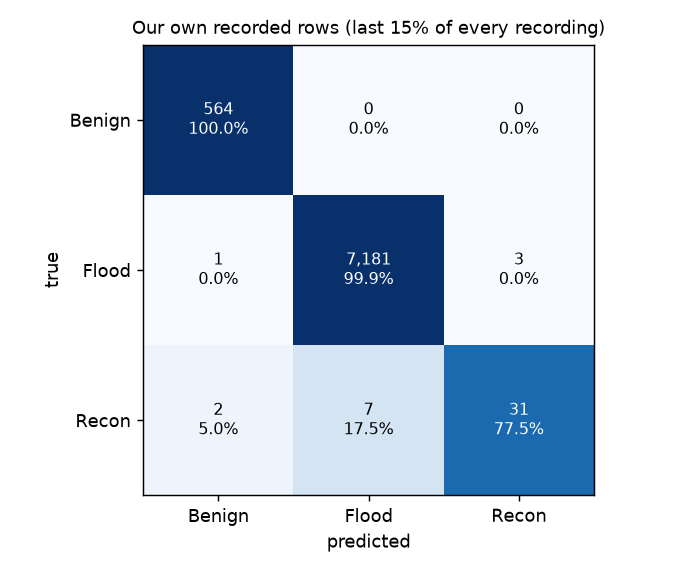
\includegraphics[width=0.46\linewidth]{images/cm_our_rows.png}
\hfill
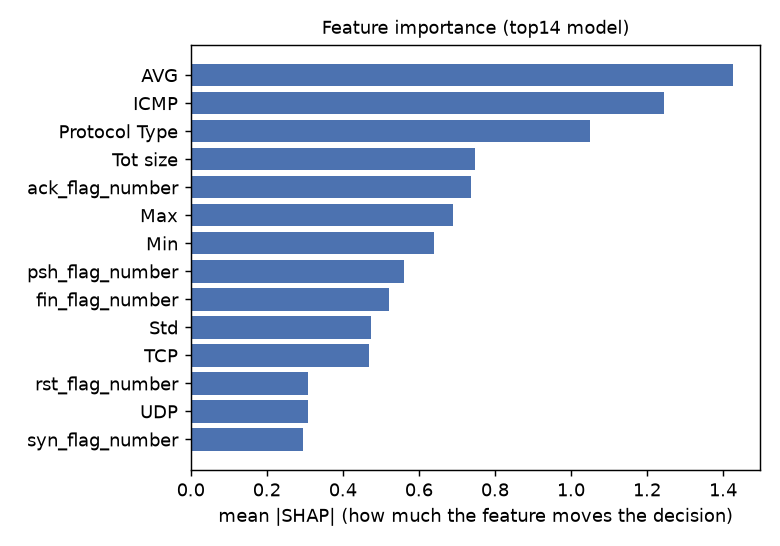
\includegraphics[width=0.5\linewidth]{images/feature_importance.png}
\caption{Left: confusion matrix on our own traffic. Right: feature importance of the deployed model (mean
$|$SHAP$|$ and gain): packet sizes and protocol dominate; the TCP flags separate flood types.}
\end{figure}

\subsection{Training on the full dataset}

\begin{center}
\small
\begin{tabular}{lcccccc}
\toprule
Training share & Macro-F1 & Binary F1 & Recon recall & Size & Train & Predict \\
\midrule
\dep 20\% (deployed recipe) & 0.760 & 0.997 & 0.291 & 918 KB & 7 s & 0.10 ms \\
100\% (4,546,831 rows) & 0.759 & 0.997 & 0.290 & 810 KB & 33 s & 0.07 ms \\
\bottomrule
\end{tabular}
\end{center}

Five times more data gives the same scores: the 20\% sample is sufficient. (The 20\% row is a retrain for this
comparison; the deployed file scores 0.760 at 974 KB.)

% =====================================================================================================
\section{Research questions}

\subsection{RQ1: number of features}

SHAP ranking from the full LightGBM, retrain with the top-$k$ features, full test split. IAT excluded, so the full
model has 45 features.

\begin{center}
\small
\begin{tabular}{lccccccc}
\toprule
Task, training data & 5 & 10 & 15 & 20 & 25 & 30 & 45 \\
\midrule
8-class, 20\% sample & 0.568 & 0.645 & 0.675 & 0.676 & 0.676 & \textbf{0.685} & 0.705 \\
3-class, 20\% sample & 0.807 & 0.863 & \textbf{0.879} & 0.882 & 0.884 & 0.884 & 0.885 \\
3-class, 100\% of rows & 0.836 & \textbf{0.874} & 0.884 & 0.886 & 0.887 & 0.889 & 0.888 \\
\midrule
Pi-computable 14 (3-class) & 0.646 & 0.754 (10) & \multicolumn{2}{l}{0.760 (all 14)} & & & \\
\bottomrule
\end{tabular}
\end{center}
{\small Bold = smallest feature count within 0.02 of the 45-feature model.}

\begin{figure}[H]
\centering
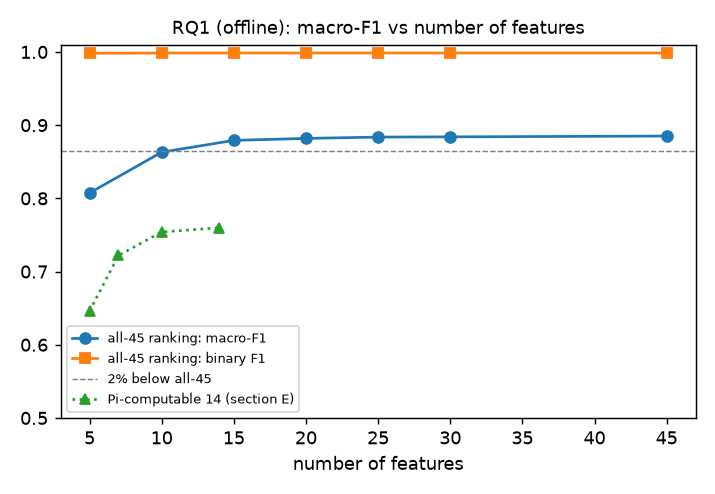
\includegraphics[width=0.56\linewidth]{images/rq1_all45.png}
\caption{RQ1: macro-F1 against the number of features (3-class task).}
\end{figure}

\answer{30 of 45 features keep the 8-class model within 2\%; for our 3-class task 15 suffice (10 with all rows).
On the gateway only 14 features are computable identically; 10 of them stay within 1\% of all 14. The remaining gap
to the 45-feature model is almost entirely the Recon class.}

\subsection{RQ2: compressed models}

Binary task; latency per window measured on the laptop (the Pi is about 3--4$\times$ slower).

\begin{center}
\small
\begin{tabular}{llrrr}
\toprule
Model & Compression & Size (KB) & Macro-F1 & Latency (ms) \\
\midrule
LightGBM & original & 6,667 & 0.945 & 0.710 \\
LightGBM & pruned (150 rounds) & 260 & 0.917 & 0.681 \\
LightGBM & pruned $\rightarrow$ ONNX & 157 & 0.917 & 0.019 \\
Random Forest & pruned (30 trees, d 12) $\rightarrow$ ONNX & 859 & 0.909 & 0.012 \\
MLP & ONNX fp32 & 57 & 0.916 & 0.010 \\
MLP & ONNX INT8 & \textbf{19} & 0.915 & 0.012 \\
1D-CNN & ONNX fp32 & 80 & 0.879 & 0.034 \\
1D-CNN & ONNX INT8 & 28 & 0.880 & 0.025 \\
\bottomrule
\end{tabular}
\end{center}

On the Pi (2,000 windows, one at a time): earlier 7~MB model 1.88~ms per window; small model 1.09~ms; deployed model
0.7--1.4~ms live.

\answer{Per megabyte the INT8 MLP is best (19 KB, no accuracy lost to quantization); per millisecond the ONNX models
are fastest. We deploy the pruned LightGBM: it meets every target on the Pi and is the only model with exact,
millisecond TreeSHAP. INT8 reduced the networks' size, not their single-window latency.}

\subsection{RQ3: explanations on the gateway}

\begin{center}
\small
\begin{tabular}{lrr}
\toprule
Model on the Raspberry Pi & SHAP per alert & Target \\
\midrule
Earlier large model (7 MB) & 45.65 ms & $<$ 50 ms \\
Small model & 2.59 ms & $<$ 50 ms \\
\dep Deployed model, live under attack & \textbf{5--14 ms} & $<$ 50 ms \\
\bottomrule
\end{tabular}
\end{center}

\answer{Yes. LightGBM's built-in TreeSHAP (\texttt{pred\_contrib=True}) produces the top-3 features of every alert in
5--14 ms on the Pi, 4--10$\times$ under target; model size matters (7 MB: 46 ms, $<$ 1 MB: 3 ms).}

% =====================================================================================================
\section{Four-classifier benchmark}

45 features, 20\% training sample, full test split; latency per row on the laptop; ``edge'' = compressed version.

\begin{center}
\small
\begin{tabular}{llrrrr}
\toprule
Task & Model & Accuracy & Macro-F1 & Size (KB) & Latency (ms) \\
\midrule
Binary & Random Forest & 0.993 & 0.932 & 7,291 & 4.56 \\
& LightGBM & 0.994 & \textbf{0.942} & 3,405 & 0.09 \\
& MLP & 0.992 & 0.928 & 187 & 0.13 \\
& 1D-CNN & 0.993 & 0.935 & 261 & 0.27 \\
& LightGBM edge & 0.993 & 0.935 & 581 & 0.06 \\
\midrule
8-class & Random Forest & 0.905 & 0.688 & 39,438 & 4.74 \\
& LightGBM & 0.908 & \textbf{0.702} & 13,720 & 0.26 \\
& MLP & 0.897 & 0.681 & 190 & 0.11 \\
& 1D-CNN & 0.904 & 0.686 & 264 & 0.25 \\
& LightGBM edge & 0.901 & 0.669 & 907 & 0.07 \\
\midrule
34-class & Random Forest & 0.887 & \textbf{0.649} & 54,635 & 4.50 \\
& LightGBM & 0.888 & 0.638 & 13,619 & 0.24 \\
& MLP & 0.881 & 0.642 & 203 & 0.12 \\
& 1D-CNN & 0.871 & 0.616 & 277 & 0.24 \\
& MLP edge (INT8) & 0.881 & 0.652 & 62 & 0.39 \\
\bottomrule
\end{tabular}
\end{center}

All four families end up close (8-class 0.68--0.70, 34-class 0.62--0.65): the limit is the data (web, brute force,
spoofing and DoS-vs-DDoS look alike in these features), not the model type. LightGBM is the fastest and the only one
with exact fast explanations, which made it the deployed choice.

% =====================================================================================================
\section{Live deployment}

\subsection{Live attacks on the real gateway}

Raspberry Pi~4, three NodeMCU sensors, attacks from the laptop (hping3, nmap, mosquitto\_pub) and from the NodeMCU
botnet; IPS enabled.

\begin{center}
\small\setlength{\tabcolsep}{4pt}
\begin{tabular}{llll}
\toprule
Attack & Alert & Conf. & Top-3 SHAP reasons \\
\midrule
SYN flood & DoS flood & 0.96 & Min, Std, ack\_flag\_number \\
UDP flood & DoS flood & 1.00 & Protocol Type, Min, UDP \\
ICMP flood & DoS flood & 1.00 & ICMP, Min, ack\_flag\_number \\
ACK flood & DoS flood & 0.98 & Min, Max, Std \\
PSH-ACK flood & DoS flood & 1.00 & psh\_flag, Min, Max \\
RST-FIN flood & DoS flood & 1.00 & fin\_flag, Min, rst\_flag \\
Port scan & Recon (model + rule) & 0.99 / 1.00 & AVG, Tot size, Max \\
Version scan & Recon & 0.99 & AVG, Tot size, Max \\
MQTT brute force & BruteForce (rule) & 1.00 & refused MQTT logins \\
Bot DDoS (TCP, UDP) & DDoS (3 senders) & 0.96--1.00 & all 3 nodes quarantined \\
\bottomrule
\end{tabular}
\end{center}

Every attack was detected and blocked with \textbf{zero false alarms} on the three sensors. Two findings from the
lab: (i) the college Wi-Fi blocks broadcast, so bot commands are sent to each node's IP; (ii) ARP spoofing could not
be exercised there, because the access point rewrites spoofed ARP replies before they reach the gateway (verified
with \texttt{tcpdump}); the ARP rule was validated in the Docker testbed.

\subsection{Dashboard}

\begin{figure}[H]
\centering
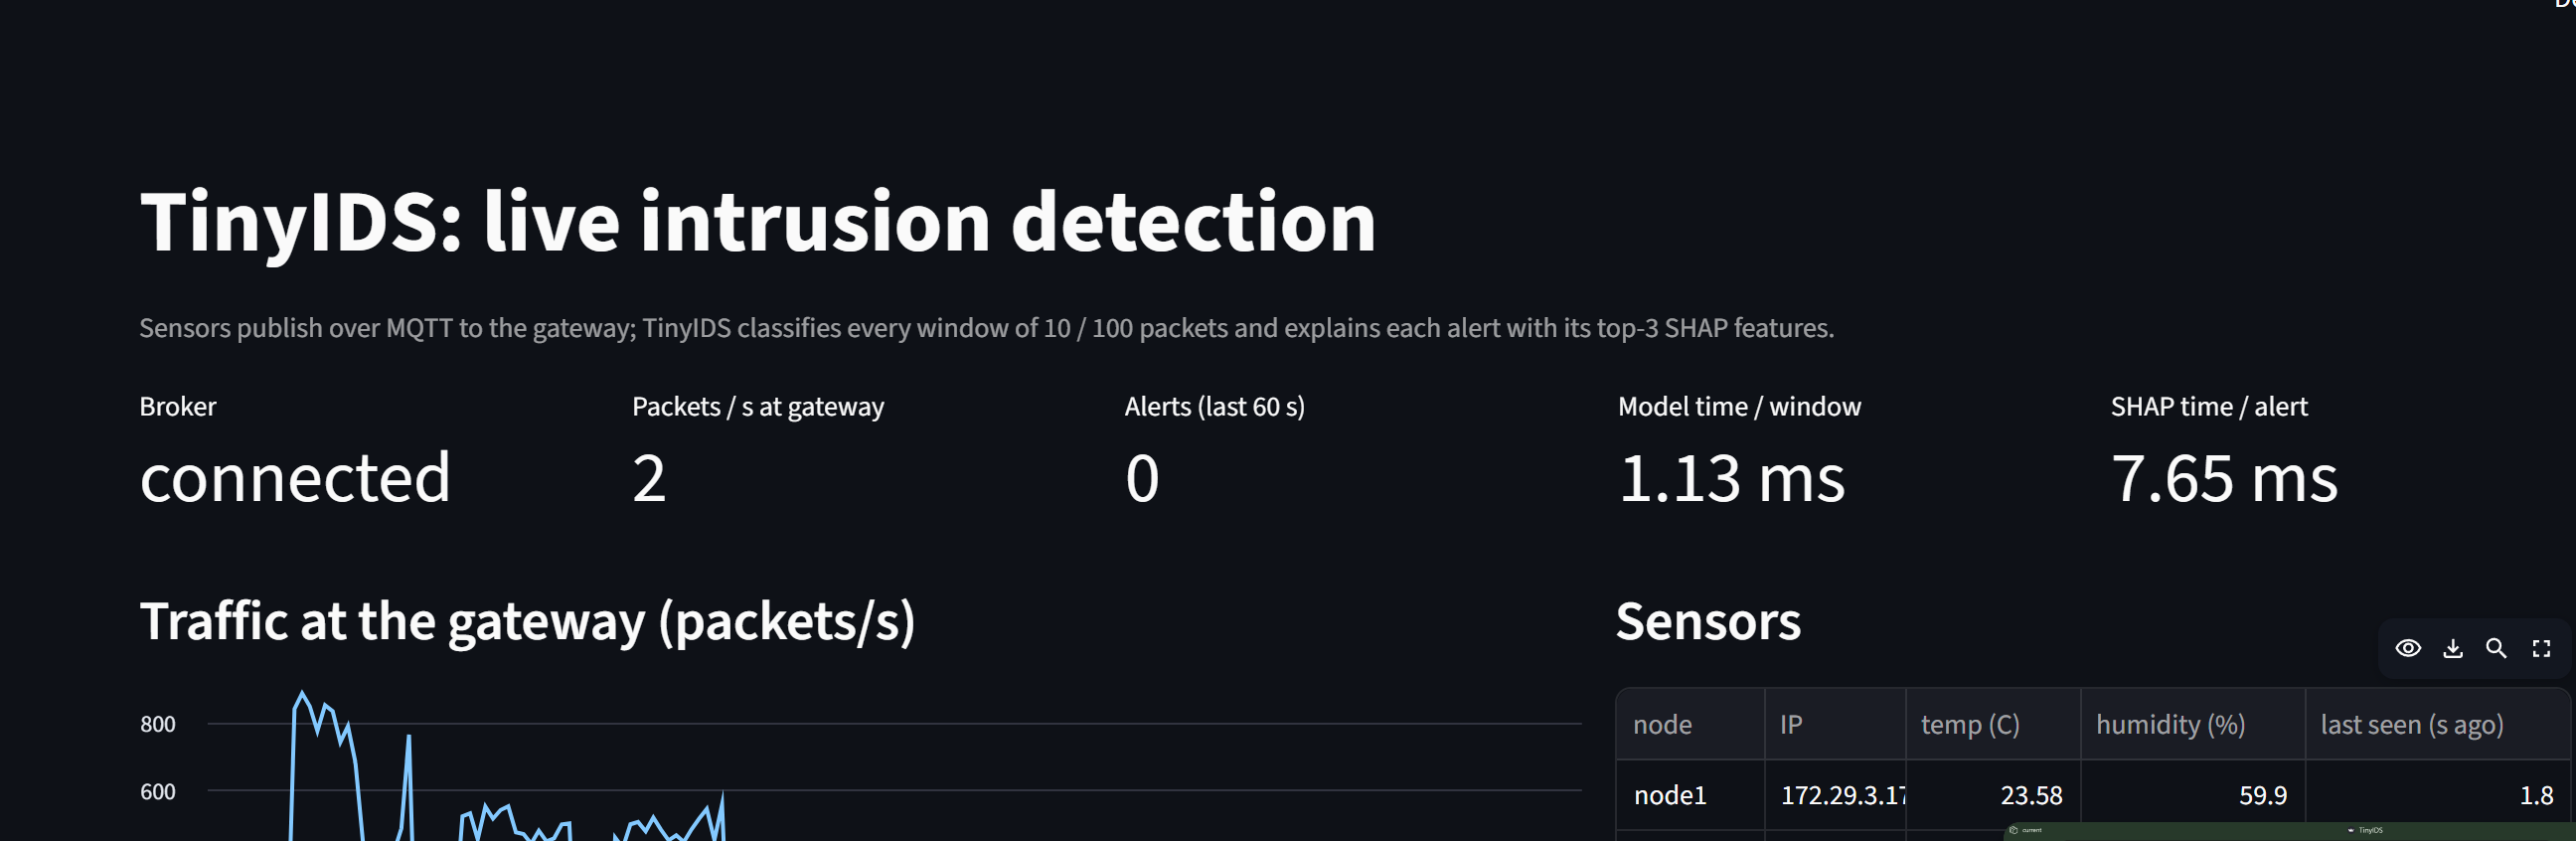
\includegraphics[width=\linewidth]{images/screens/lab_overview.png}
\caption{Dashboard on the real gateway: broker status, packets per second, model time per window and SHAP time
per alert, the traffic chart and the three sensors.}
\end{figure}

\begin{figure}[H]
\centering
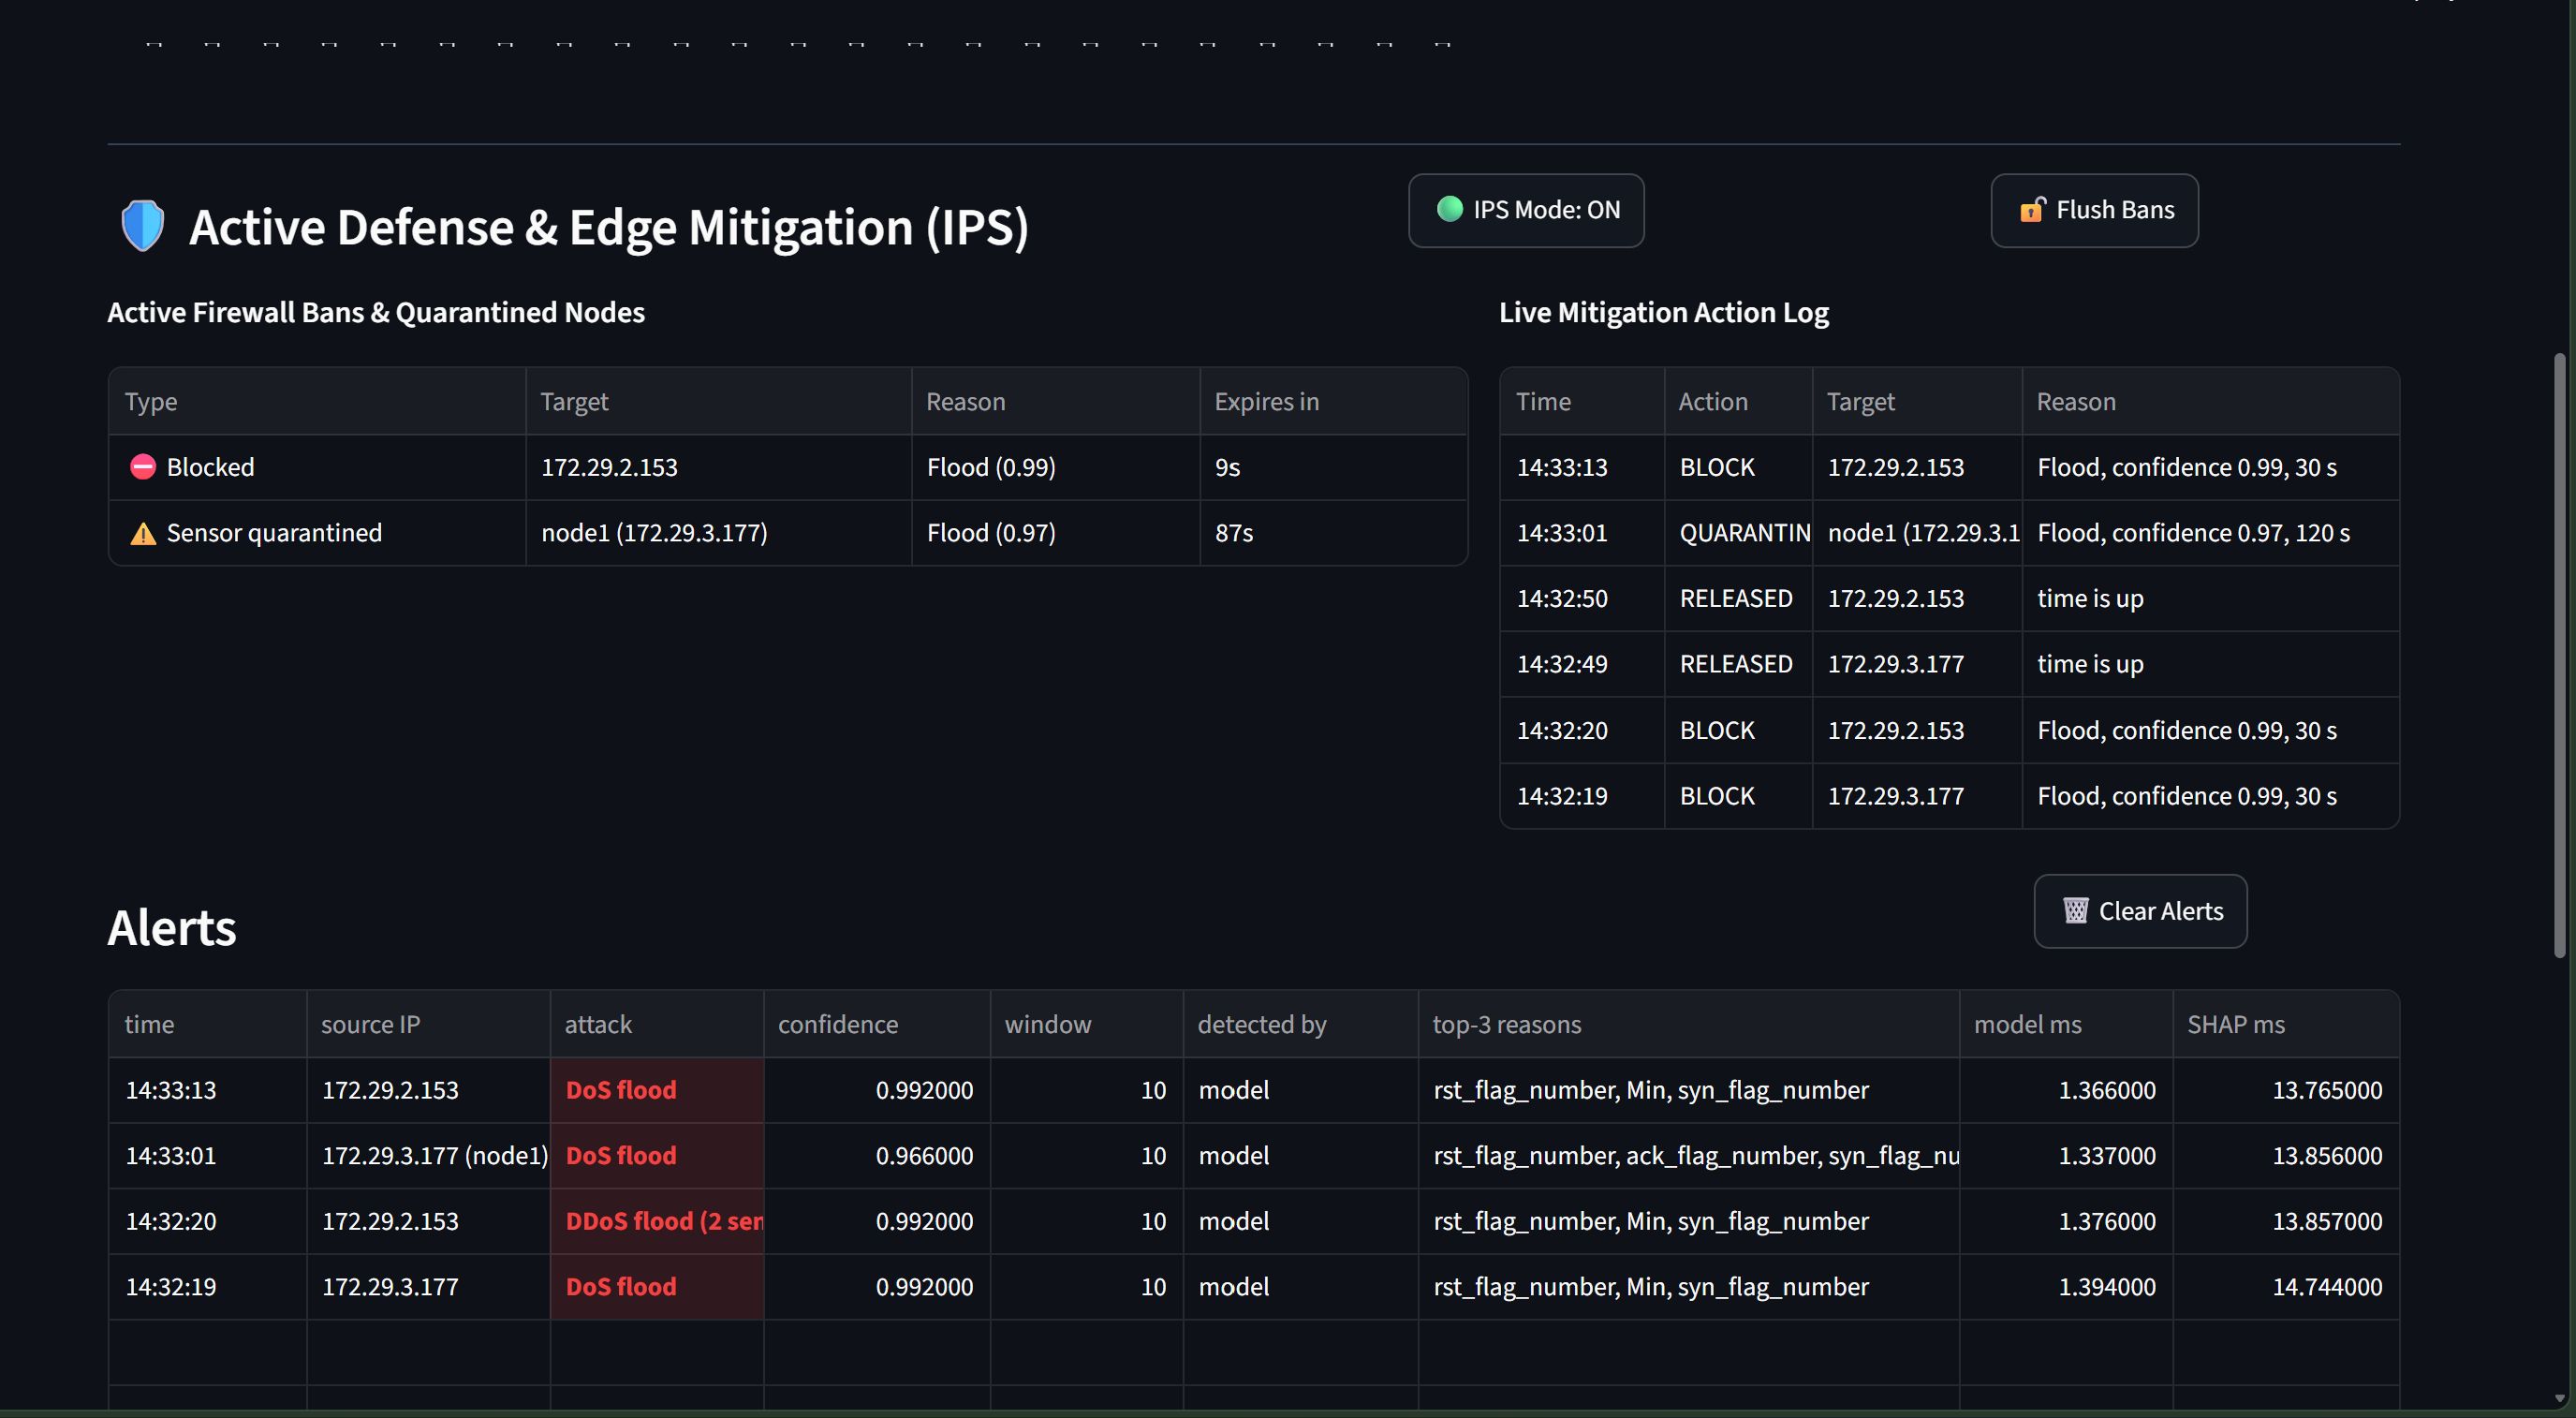
\includegraphics[width=\linewidth]{images/screens/lab_mitigation_alerts.png}
\caption{Live mitigation on the real gateway: an attacker blocked and a compromised sensor quarantined, the action
log, and the alert table with the top-3 reasons and timings.}
\end{figure}

\begin{figure}[H]
\centering
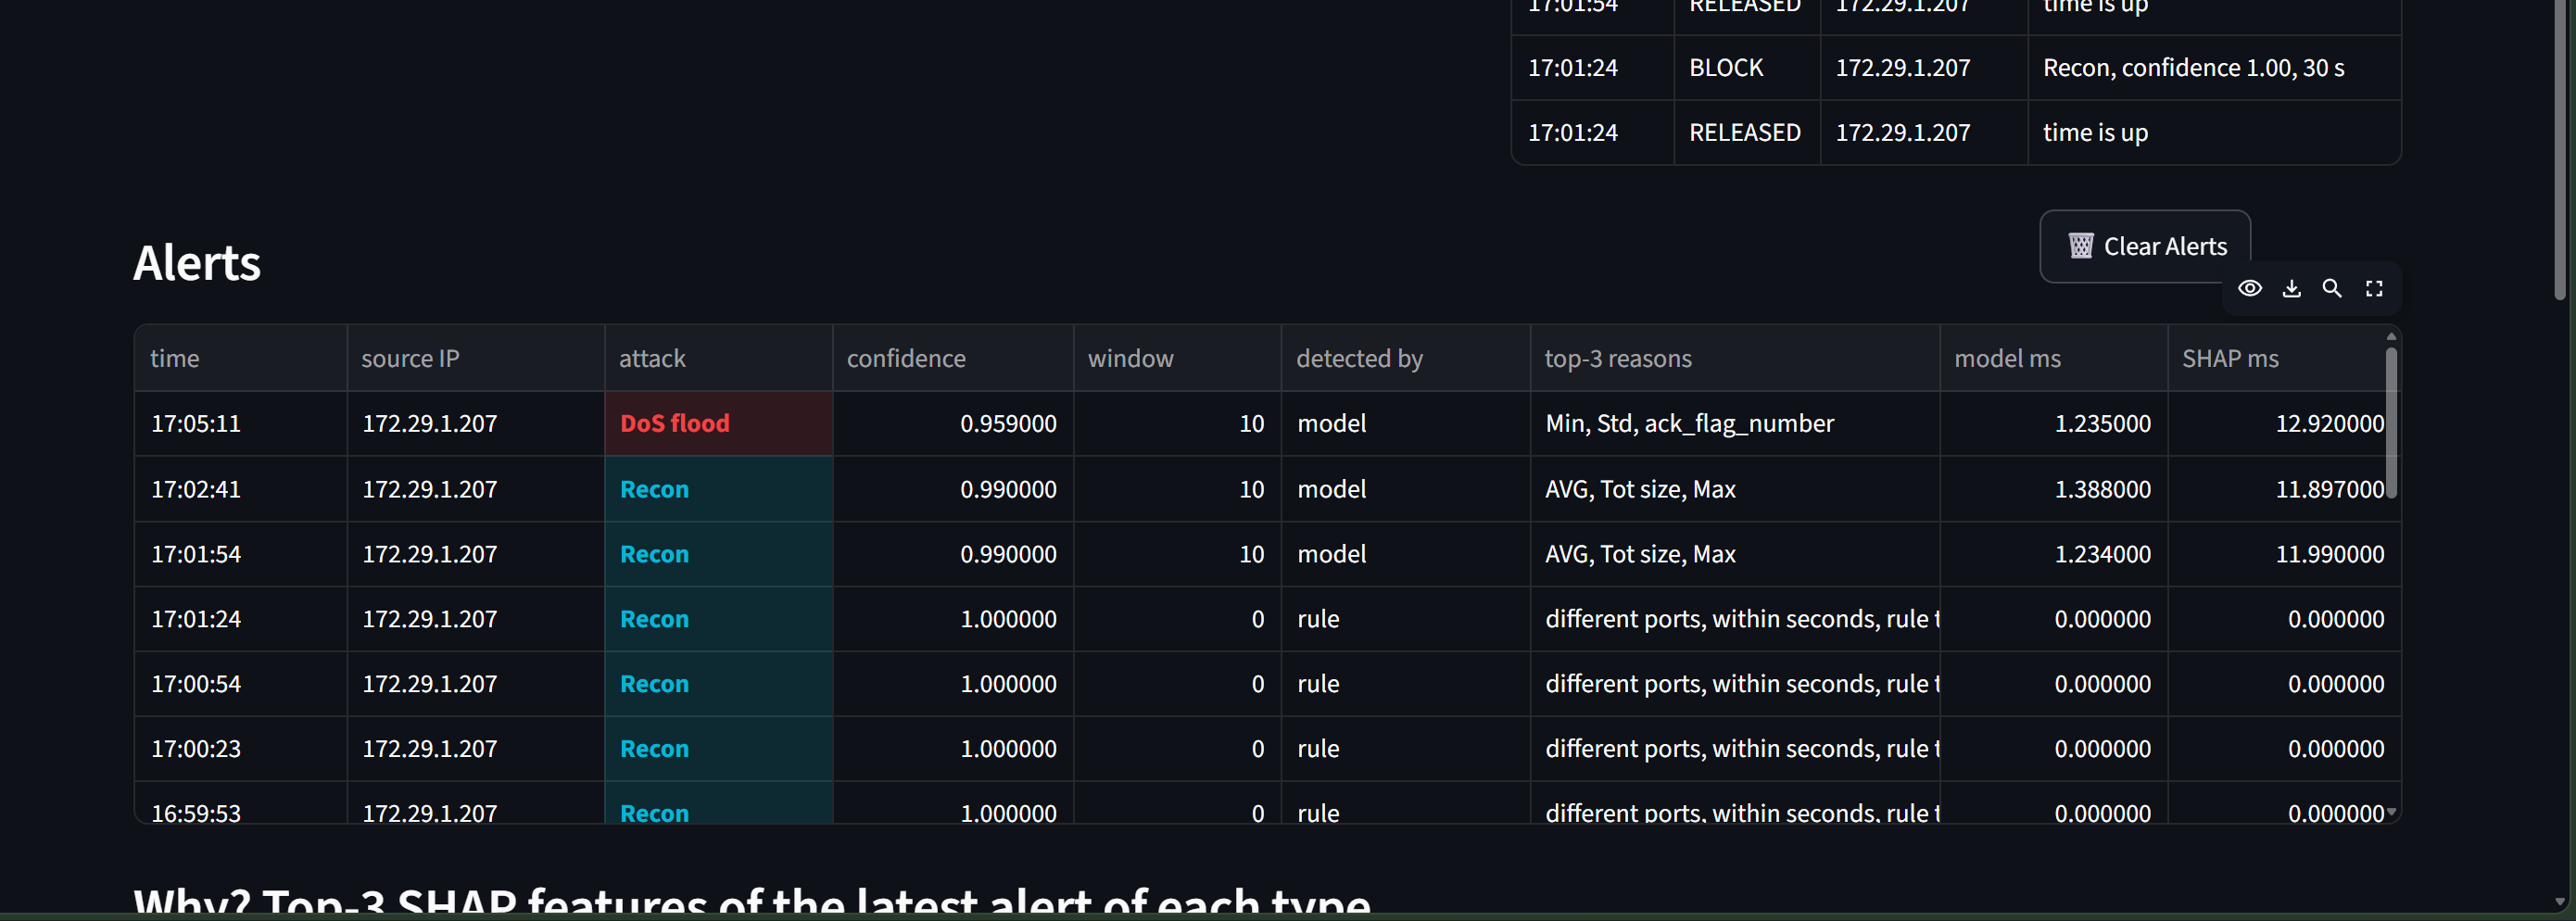
\includegraphics[width=\linewidth]{images/screens/lab_portscan_alerts.png}
\caption{Port scans on the real gateway, detected by the port-scan rule (``different ports'') and by the model
(Recon, reasons AVG, Tot size, Max).}
\end{figure}

\begin{figure}[H]
\centering
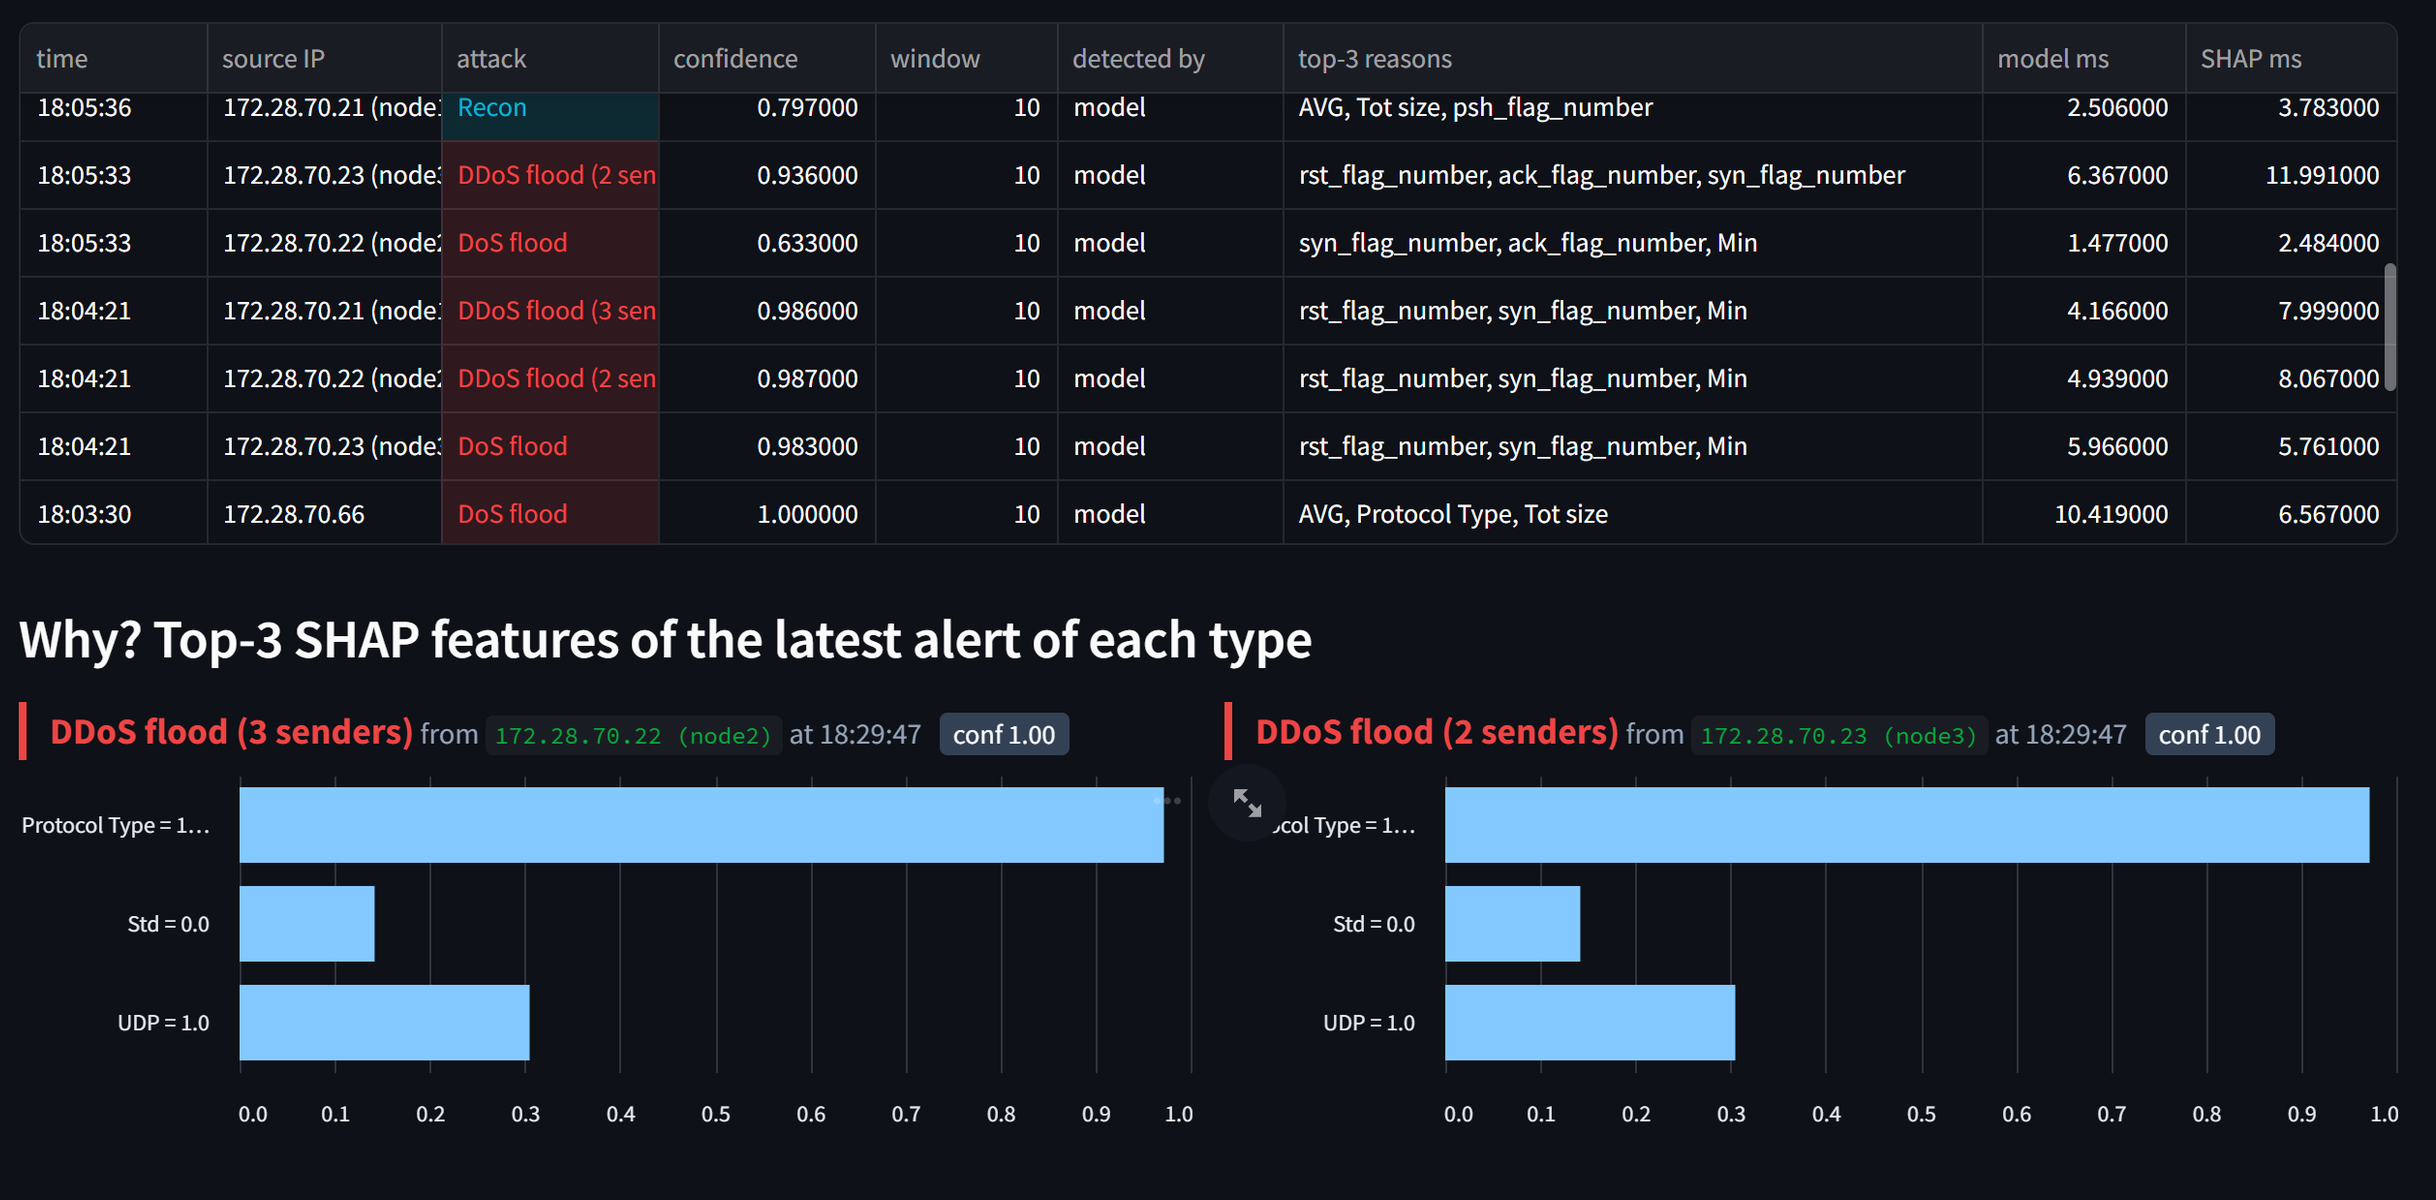
\includegraphics[width=0.92\linewidth]{images/screens/docker_shap.png}
\caption{Alert table and SHAP charts (feature = value in the window) during a botnet DDoS, Docker testbed.}
\end{figure}

% =====================================================================================================
\section{Limitations and future work}

\begin{itemize}
  \item \textbf{Recon} is the weak class on the dataset (recall 0.29), and a fast scan can be named ``Flood'' when
        the model fires before the port-scan rule; a lower port threshold or more recorded scans would help.
  \item \textbf{Energy} per inference was not measured (no USB power meter), and the RQ2 benchmark of all
        compressed models has been prepared but not yet run on the Pi.
  \item \textbf{Low-rate DDoS} and fragmentation floods are only partly covered; an entropy-based rule over all
        senders is a natural extension.
  \item \textbf{One shared MQTT password}: per-device users, topic ACLs and TLS would harden the broker.
  \item NodeMCU (ESP8266) boards were used instead of ESP32; they fill the same role.
\end{itemize}

% =====================================================================================================
\section{Conclusion}

TinyIDS shows that useful, explainable intrusion detection fits on a Raspberry Pi gateway: a 974 KB LightGBM model
on 14 carefully chosen features reaches a binary F1 of 0.997 on CICIoT2023, decides in about a millisecond,
explains every alert in 5--14 ms, and together with simple rules and automatic firewall mitigation stopped every
live attack in our testbed without a single false alarm on the sensors. The study also shows where the limits lie:
reconnaissance traffic is hard to separate from benign traffic with header features alone, and feature validity
(computing features exactly as the training data did) matters more for live performance than model choice.

% =====================================================================================================
\section*{References}
\small
\begin{enumerate}[label={[\arabic*]}]
  \item E.~C.~P. Neto et al., ``CICIoT2023: A Real-Time Dataset and Benchmark for Large-Scale Attacks in IoT
        Environment,'' \emph{Sensors}, vol.~23, no.~13, 5941, 2023.
  \item Canadian Institute for Cybersecurity, ``CIC IoT Dataset 2023,'' University of New Brunswick.
  \item ``Realguard: A Lightweight Network Intrusion Detection System for IoT Gateways,'' \emph{Sensors}, 2022.
  \item ``Think Fast: Real-Time IoT Intrusion Reasoning Using IDS and LLMs at the Edge Gateway,'' arXiv:2511.18230.
  \item ``Derived CICIoT 2023 datasets,'' Mendeley Data.
  \item S.~M. Lundberg and S.-I. Lee, ``A Unified Approach to Interpreting Model Predictions,'' NeurIPS, 2017.
  \item G.~Ke et al., ``LightGBM: A Highly Efficient Gradient Boosting Decision Tree,'' NeurIPS, 2017.
\end{enumerate}

\end{document}
